\chapter{Symmetry and SAT}\label{chap:symmetryinsat}
\minitoc
Despite the NP-Completeness character of the SAT problem, state-of-the-art solvers are able to treat many industrial problems.
This is mainly due to the capacity of SAT solvers to prune search space using, for instance, learnt clauses.
Another way to accelerate the solving is the exploitation of symmetries.
These are common in real life. \\
Consider the problem of searching for a pattern in butterfly wings.
Most butterflies have an identical pair of wings. After checking that both wings are symmetric
(process called symmetry detection), the pattern can be searched for only one wing. Searching this pattern in the other wing is useless (process called symmetry exploitation). 
In this chapter, we show how to detect that a given formula has symmetries and how to
exploit them to accelerate the solving in the SAT context.
%Some instances exhibit symmetries and not taking them into account forces solvers to needlessly explore isomorphic search space.  

\section{Group theory basics} 
Since symmetries belong to a branch of mathematics called group theory, this section gives us an overview.
\subsection{Groups}

%\begin{theoo}[Pythagoras' theorem]
% In a right triangle, the square of the hypotenuse is equal to the sum of the squares of the catheti.
% $$a^2+b^2=c^2$$
%\end{theoo}
\begin{definition}[Group]
 A \emph{group} is a structure $\langle G, * \rangle$, where $G$ is a non-empty set and $*$ a binary
 operation such that the following axioms are satisfied:
 \begin{itemize}[noitemsep,nolistsep]
  \item \emph{associativity}: $\forall a, b, c \in G, (a * b) * c = a * (b * c)$
  \item \emph{closure}: $\forall a, b \in G, a * b \in G$.
  \item \emph{identity}: $\forall a \in G, \exists e$ such that $ a * e = e * a = a$
  \item \emph{inverse}:  $\forall a \in G, \exists b \in G$, commonly denoted $a^{-1}$, such that
  $a * a^{-1} = a^{-1} * a = e$
 \end{itemize}
\end{definition}
Note that, \emph{commutativity} (i.e. $\ a * b = b * a$, for $a, b \in G$) is not a required axiom.
If it satisfies it, the group is said \emph{abelian}.
The last definition leads to important properties: i) uniqueness of the identity element. 
To prove this property, assume $\langle G, * \rangle$ a group with two identity elements $e$ and $f$ 
then $ e = e * f = f$.
ii) Uniqueness of the inverse element. To prove this property, suppose that an element $a$ has two inverses,
denoted $b$ and $c$ in groups $\langle G, * \rangle$, then,\\
 $\begin{array}{lcll}     
b & = & b * e & \\
& = & b * (a * c) & c \text{ is an inverse of } a, \text{so } e = a * c\\
& = & (b * a) * c &   \text{\emph{associativity} rule}\\
& = & e * c       & b \text{ is an inverse of } a, \text{so } e = a * b\\
& = & c           &   \text{\emph{identity} rule}
\end{array}$


The structure $\langle G, * \rangle$ is denoted simply $G$ when clear from the context that G is a group
with a binary operation. In this thesis, we only consider \emph{finite} groups, i.e. groups with a finite number of elements.
\begin{definition}[Subgroup]
Given a group $G$, a \emph{subgroup} is a non-empty subset of $G$ which is also a group with 
the same binary operation. We denote $H \leq G$, the subgroup $H$ of $G$.
\end{definition}
A group has at least two subgroups: 
\begin{enumerate}[topsep=0pt,nolistsep]
 \item \emph{trivial} subgroup: the subgroup composed of the identity element $\{e\}$. (All other subgroups are \textit{non-trivial})
 \item \emph{improper} subgroup: the subgroup composed of itself. (All other subgroups are \emph{proper}).
\end{enumerate}
%i) ; ii)
%\subsubsection{Generators of a group}
\begin{definition}[Generators of a group]
 If every element in a group G can be expressed as a linear combination
 of a set of elements S = $\{g_1, g_2, ..., g_n \}$ then we say that $G$ is 
 \textit{generated by S}. This is denoted by G = $\langle S \rangle$ =
 $\langle \{g_1, g_2, ..., g_n \} \rangle$ 
\end{definition}
In other words, to obtain the group, it is sufficient to compose all permutations in the generators set until a fix point.
So the generators are a compact representation of a group.
\subsection{Permutation group}
\begin{definition}[Permutation]
 A \emph{permutation} is a bijection from a set $X$ to itself.
\end{definition}
Example: given a set $X = \{x_1, x_2, x_3, x_4, x_5, x_6\}$,
\begin{center}
$g = ${\Bigg( \begin{tabular}{cccccc}
  $x_1$ & $x_2$ & $x_3$ & $x_4$ & $x_5$ & $x_6$\\
  $x_2$ & $x_3$ & $x_1$ & $x_4$ & $x_6$ & $x_5$
 \end{tabular} \Bigg)}\\
\end{center}
In this example, $g$ is a permutation that maps $x_1$ to $x_2$, $x_2$ to $x_3$, $x_3$ to $x_1$, $x_4$ to $x_4$, $x_5$ to $x_6$ and $x_6$ to $x_5$.
Permutations are generally written in \emph{cycle notation}, the self-mapped elements are omitted.
So the permutation in cycle notation will be 
\begin{center}
 $g$ = ($x_1 \enskip x_2 \enskip x_3$) ($x_5 \enskip x_6$)
\end{center}
\begin{definition}[Support of a permutation]
 The \emph{support} of the permutation $g$, noted $\mathit{\support_{g}}$, is the set of elements that are not mapped to themselves:
 \begin{center}
  $\support_{g} = \{ x \in X \mid g.x \neq x\}$
 \end{center}
\end{definition}

\hakan{REVOIR}
\begin{definition}[Stabilized variable over permutation]
 A variable $x$ is \emph{stable} by a permutation $g$  iff $x \notin \support_g$.
\end{definition}
 
%\hakan{mettre ailleurs A clause $\omega$ is \emph{stabilized} by a permutation $g$ if $\omega \cap \support_g = \emptyset$.}
\begin{definition}[Permutation Group]
 A set of permutations of a given set $X$ form a group $G_X$ with the composition operation ($\circ$) called \emph{permutation group}.
\end{definition}
\begin{definition}[Symmetric Group]
The set of \textbf{all} permutations of a set $X$ is the \emph{symmetric group} of $X$ and is noted \Group($X$).
\end{definition}
%The \emph{symmetric group} is the set of all possible permutations of a set $X$ and noted \Group($X$).
%
%So, $G_X \leq \Group(X)$. 
%A set of permutations $P$ is a set of \emph{generators} of a group $G$ if each permutation of $G$
%can be expressed as a composition of permutations in $P$. 
A permutation group $G$ induces an \emph{equivalence relation} on the set of elements $X$ being
permuted. Two elements $x_1, x_2 \in X$ are equivalent if there exists a permutation $g \in G$ such that
$g.x_1 = x_2$. The equivalence relation partitions $X$ into \emph{equivalence classes} referred to
as the \emph{orbits} of $X$ under $G$. The orbit of an element $x$ under group $G$ (or simply orbit of $x$ when clear
from the context) is the set. $[x]_G = \{g.x \mid g \in G\}$
\section{Symmetries in SAT}
The previous mathematical definitions of group theory can be applied to a CNF formula.
The symmetric group of permutations of $\Vars$ (i.e., bijections from $\Vars$ to $\Vars$) is noted
$\Group(\Vars)$. The group $\Group(\Vars)$ naturally acts on the set of literals: for $g
\in \Group(\Vars)$ and a literal $\ell \in \Lits $, $g.\ell = g(\ell)$ if $\ell$ is a
positive literal, and $g.\ell = \neg g(\neg \ell)$ if $\ell$ is a negative literal.
The group $\Group(\Vars)$ acts on  assignments (possibly partial) of $\Vars$ as follows: 
\begin{center}
 $\forall g \in \Group(\Vars)$, $ \forall \alpha \in \Assignments(\Vars)$, $g.\alpha = \{ g.\ell ~|~ \ell \in \alpha \}$.
\end{center}
% We say that $g\in \Group(\Vars)$ is a \textit{symmetry of $ \varphi$} if the following conditions holds:
%\begin{itemize}[topsep=0em]
% \item permutation fixes the formula, $g.\varphi =  \varphi$: 
% \item $g$  commutes with the negation: $g.\neg l  = \neg (g.l)$
%\end{itemize}
The set of symmetries of $\varphi$ is noted $G_{\varphi}$ and is a subgroup of $\Group(\Vars)$.
Symmetry of a formula $\varphi$ preserves the satisfaction, for every \emph{complete} assignment $\alpha$:
\begin{center}
 $\alpha \models \varphi\Leftrightarrow g.\alpha \models \varphi$
\end{center}
%$
%\neg x_1 \neg x_2 \\
%\neg x_1 \neg x_3 \\
%\neg x_2 \neg x_3 \\
%\neg x_4 \neg x_5 \\
%\neg x_4 \neg x_6 \\
%\neg x_5 \neg x_6 \\
%\neg x_7 \neg x_8 \\
%\neg x_7 \neg x_9 \\
%\neg x_8 \neg x_9 \\
%\neg x_{10} \neg x_{11} \\
%\neg x_{10} \neg x_{12} \\
%\neg x_{11} \neg x_{12} \\
%x_1 x_4 x_7 x_{10} \\
%x_2 x_5 x_8 x_{11} \\
%x_3 x_6 x_9 x_{12} \\
%x_1 x_6 x_8 x_{10} \\
%x_2 x_4 x_9 x_{11} \\
%x_3 x_5 x_7 x_{12} \\
%x_1 x_5 x_9 x_{10} \\
%x_2 x_6 x_7 x_{11} \\
%x_3 x_4 x_8 x_{12} \\
%$
%\begin{figure}[!htbp]
% 
\begin{minipage}[c]{0.6\linewidth}
\begin{tikzpicture}[level/.style={sibling distance=60mm/#1},every node/.style={scale=0.6}, scale=0.6]
  \tikzstyle{trans}=[thick, ->, sloped]
  \tikzstyle{unsat}=[thick,fill=purple,scale=1.5]
  \tikzstyle{sat}=[thick,fill=hgreen,scale=1.5]
  \tikzstyle{alpha}=[sibling distance=0pt,level distance=20pt]
  
\node [circle,draw] (x1) {$x_1$}
  child {node [circle,draw] (x2_1) {$x_2$}
    child {node [circle,draw] (x3_1) {$x_3$}
      child {node[unsat]  (xn_1) {}
   	     child[alpha] { node (a1) {$\alpha_1$} edge from parent[draw=none]}}
      child {node[sat] (xn_2) {}
   	     child[alpha] { node (a1) {$\alpha_2$} edge from parent[draw=none]}}
    }
    child {node [circle,draw] (x3_2) {$x_3$}
      child {node[sat] (xn_3) {}
  	     child[alpha] { node (a1) {$\alpha_3$} edge from parent[draw=none]}}
      child {node[unsat] (xn_4) {}
   	     child[alpha] { node (a1) {$\alpha_4$} edge from parent[draw=none]}}
    }
  }
  child {node [circle,draw] (x2_2) {$x_2$}
    child {node [circle,draw] (x3_3) {$x_3$}
      child {node[sat] (xn_5) {}
   	     child[alpha] { node (a1) {$\alpha_5$} edge from parent[draw=none]}}
      child {node[unsat] (xn_6) {}
   	     child[alpha] { node (a1) {$\alpha_6$} edge from parent[draw=none]}}
    }
  child {node [circle,draw] (x3_4) {$x_3$}
    child {node[unsat] (xn_7) {}
   		child[alpha] { node (a1) {$\alpha_7$} edge from parent[draw=none]}}
    child {node[unsat] (xn_8) {}
    	child[alpha] { node (a1) {$\alpha_8$} edge from parent[draw=none]}}
  }};


\path (x1)   -- (x2_1) node [midway, fill=white] {$0$};
\path (x2_1) -- (x3_1) node [midway, fill=white] {$0$};
\path (x3_1) -- (xn_1) node [midway, fill=white] {$0$};
\path (x3_2) -- (xn_3) node [midway, fill=white] {$0$};
\path (x2_2) -- (x3_3) node [midway, fill=white] {$0$};
\path (x2_2) -- (x3_4) node [midway, fill=white] {$1$};
\path (x1)   -- (x2_2) node [midway, fill=white] {$1$};
\path (x3_1) -- (xn_2) node [midway, fill=white] {$1$};
\path (x2_1) -- (x3_2) node [midway, fill=white] {$1$};
\path (x3_2) -- (xn_4) node [midway, fill=white] {$1$};
\path (x3_3) -- (xn_5) node [midway, fill=white] {$0$};
\path (x3_3) -- (xn_6) node [midway, fill=white] {$1$};
\path (x3_4) -- (xn_7) node [midway, fill=white] {$0$};
\path (x3_4) -- (xn_8) node [midway, fill=white] {$1$};

%\path (xn_8) -- (x6_3) node [midway, fill=white] {$0$};
%\path (xn_8) -- (x6_4) node [midway, fill=white] {$1$};

\end{tikzpicture}
\end{minipage}
\begin{minipage}[c]{0.23\linewidth}
           \footnotesize
		\begin{itemize}
			\item[] $\omega_1 = \{x_1, x_2, x_3\}$ \\
			\item[] $\omega_2 = \{\neg x_1, \neg x_2 \}$\\
			\item[] $\omega_3 = \{\neg x_1, \neg x_3 \}$\\
			\item[] $\omega_4 = \{\neg x_2, \neg x_3 \}$\\
		\end{itemize}
\end{minipage}

% \caption{Example of symmetries}
%\end{figure}

%The symmetric group of permutations of $\Vars$ (i.e. bijections from $\Vars$ to $\Vars$) is noted
%$\Group(\Vars)$. The group $\Group(\Vars)$ naturally acts on the set of literals: for $g
%\in \Group(\Vars)$ and a literal $\ell \in \Lits $, $g.\ell = g(\ell)$ if $\ell$ is a
%positive literal, $g.\ell = \neg g(\neg \ell)$ if $\ell$ is a negative literal.
%The group $\Group(\Vars)$ also acts on (partial) assignments of $\Vars$ as follows: for
%$g \in \Group(\Vars)$, $\alpha \in \Assignments(\Vars)$, $g.\alpha = \{ g.\ell ~|~ \ell \in \alpha \}$. Let $\varphi$ be a formula, and $g \in \Group(\Vars)$.
% We say that $g\in \Group(\Vars)$ is a
%symmetry of $ \varphi$ if for every \emph{complete} assignment $\alpha$:
%The set of symmetries of $\varphi$ is noted $S(\varphi) \subseteq \Group(\Vars)$.
%
%$\alpha \models \varphi \leftrightarrow g.\alpha. \models \varphi$ for $g \in S(\varphi)$.
%The group $S(\varphi)$ also acts on (partial) assignments of $\Vars$ as follows: for
%$g \in S(\varphi)$, $\alpha \in \Assignments(\Vars)$, $g.\alpha = \{ g.\ell ~|~ \ell \in \alpha \}$,
%and acts also on clauses as follow g.$\omega$ = $\{g.l ~|~ l \in \omega \}$.
%
%
%The next section presents how to compute the set of \emph{generators} of a given formula.
These symmetries can be obtained either \textit{syntactically} or \textit{semantically}.
Semantic symmetries are independent of any particular representation of the problem. Conversely,
syntactic symmetries depend of the encoding of the problem and can lead to different symmetries.
 We say that $g\in \Group(\Vars)$ is a \textit{symmetry of $ \varphi$} if the following conditions hold:
\begin{itemize}[topsep=0em]
 \item permutation fixes the formula, $g.\varphi =  \varphi$: 
 \item $g$  commutes with the negation: $g.\neg l  = \neg (g.l)$
\end{itemize}
%The next section presents the detection of syntactical symmetries.
\section{Symmetry detection in SAT}
For the detection of symmetries in SAT, we first introduce the notion of graph automorphism.
Given a colored graph $Gr = (V, E, \gamma)$, with a set of vertices set $V \in  [1, n] $, a set of edges $E$ and
$\gamma$ a mapping: $V \rightarrow C$, where C is a set of \emph{colors},
an automorphism of $Gr$ is a permutation on its vertices, $aut :V \rightarrow V$,
such that:
\begin{itemize}
 \item $\forall (u, v) \in E \implies (aut.u, aut.v) \in E$
 \item $\forall v \in V, \gamma(v) = \gamma(aut.v)$
\end{itemize}
The graph automorphism problem is to find if a given graph has a non-trivial permutation group. 
The computational complexity of this algorithm is conjectured to be strictly between P and NP~\cite{kobler2012graph,toran2004hardness}.
Several tools exist to handle this problem like \saucy~\cite{katebi2010symmetry},
\bliss~\cite{JunttilaKaski:ALENEX2007}, \nauty~\cite{mckay2003nauty}, etc.
%There exists different ways to encode a SAT problem, which lead to different symmetries of this problem.
%
%When a symmetry depends on the structure of the problem, we say \emph{syntactic} symmetries. 
%In contrast, symmetries were \emph{semantic}, when it is not inherent to the encoding.
To find symmetries in a SAT problem, the formula is encoded in a colored graph
and an automorphism tool is applied on it. In particular, given a formula $\varphi$ with
$m$ clauses and $n$ variables, the graph is constructed as follows~\cite{biere2009handbook}:
\begin{itemize}
 \item \emph{clause nodes}: represent each of the $m$ clauses by a node with color 0;
 \item \emph{literal nodes}: represent each of the $l$ literals by a node with color 1;
 \item \emph{clause edges}: connect a clause to its literals by linking the corresponding  clause node and literal nodes;
 \item \emph{boolean consistency edges}: connect each pair of literals that correspond to the same variable.
\end{itemize}
\begin{figure}[!htbp]
 \begin{minipage}[c]{.2\textwidth}
  $\omega_{1} = \{ x_{1}, x_{2}, x_{3} \}$ \\
  $\omega_{2} = \{ x_{4}, x_{5}, x_{6} \}$ \\
  $\omega_{3} = \{ x_{1}, x_{4} \}$ \\
  $\omega_{4} = \{ x_{2}, x_{5} \}$ \\
  $\omega_{5} = \{ x_{3}, x_{6} \}$ \\
  $\omega_{6} = \{ \neg x_{1}, \neg x_{2} \}$ \\
  $\omega_{7} = \{ \neg x_{1}, \neg x_{3} \}$ \\
  $\omega_{8} = \{ \neg x_{2}, \neg x_{3} \}$ \\
  $\omega_{9} = \{ \neg x_{4}, \neg x_{5} \}$ \\
  $\omega_{10} = \{ \neg x_{4}, \neg x_{6} \}$ \\
  $\omega_{11} = \{ \neg x_{5}, \neg x_{6} \}$ \\
  
 \end{minipage}
 \begin{minipage}[l]{.75\textwidth}
  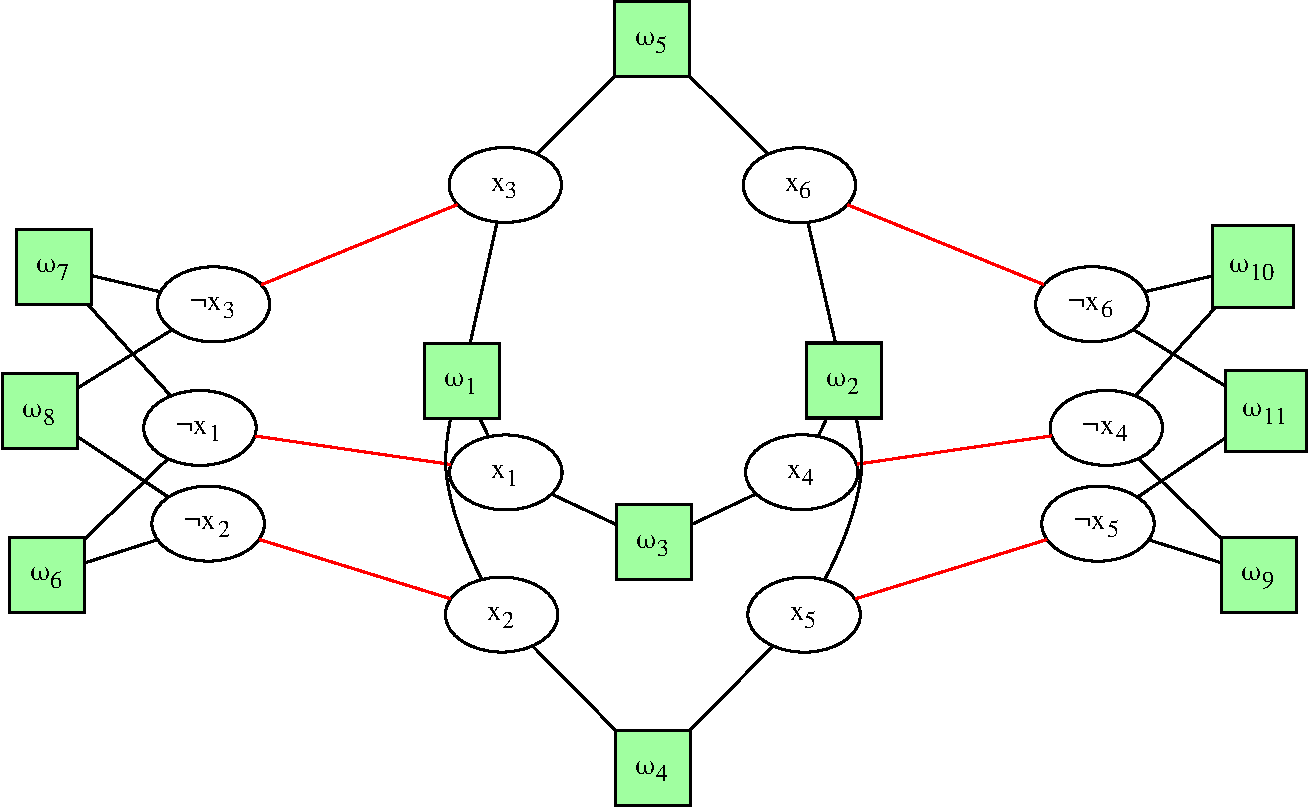
\includegraphics[width=4.3in]{cnfs/graph_cnf_no_opt-crop}
 \end{minipage}
 \caption{Example of constructed symmetry graph for a given CNF}
 \label{fig:graph_no_opt}
\end{figure}
\Cref{fig:graph_no_opt} shows the graph representation of a CNF. This problem has 6 variables and 11
clauses. So, the graph will have  12  + 11 = 33 vertices, where 12 represent the number of literal vertices (circles in the figure ) 
and 11 represents the number of clause vertices (squares in the figure). The graph will also have 6 + 24 = 30 edges, 6 
edges for Boolean consistency (red edges in the figure) and 24 edges that rely clause vertices to the literals.
% and  24 + 36 = 60 
%
%\hakan{Explication du graph + informations num nodes num edges. Probleme reel battleship
%}
%
%The battleship problems place one  ship of size *** and two ships of size* in grid 3x4 \\
%1  2  3\\
%4  5  6\\
%7  8  9\\
%10 11 12\\
%one ship per row.\\
%
%Produced graph contains and = 60 edges 
An optimization to reduce the number of graph vertices is possible. It is achieved by modeling binary clause
using graph edges instead of graph vertices.  However, in some particular cases, it can produce
spurious permutations (i.e. Boolean consistency is not respected~\cite{aloul2003solving}).
To ensure that the permutation is valid, the following condition must be satisfied:
$$\forall x \in \support_g, g.\neg x == \neg g.x$$
In other words, we check if the image of the negation of $x$ is equals to the negation of the image of $x$,
or each element $x$ in the support of the permutation.
This optimization reduces considerably the size of the 
graph, and accelerates the symmetry detection.
In the previous example, we can remove 12 nodes and 12 edges. More generally,
we can remove from the graph as many nodes and edges as those are binary clauses on the formula.
\Cref{fig:graph_opt} represents the optimized graph for the detection of automorphism.
\begin{figure}[!htbp]
 \begin{minipage}[r]{.2\textwidth}
   $\omega_{1} = \{ x_{1}, x_{2}, x_{3} \}$ \\
 $\omega_{2} = \{ x_{4}, x_{5}, x_{6} \}$ \\
 $\omega_{3} = \{ x_{1}, x_{4} \}$ \\
 $\omega_{4} = \{ x_{2}, x_{5} \}$ \\
 $\omega_{5} = \{ x_{3}, x_{6} \}$ \\
 $\omega_{6} = \{ \neg x_{1}, \neg x_{2} \}$ \\
 $\omega_{7} = \{ \neg x_{1}, \neg x_{3} \}$ \\
 $\omega_{8} = \{ \neg x_{2}, \neg x_{3} \}$ \\
 $\omega_{9} = \{ \neg x_{4}, \neg x_{5} \}$ \\
 $\omega_{10} = \{ \neg x_{4}, \neg x_{6} \}$ \\
 $\omega_{11} = \{ \neg x_{5}, \neg x_{6} \}$ \\
 \end{minipage}
 \begin{minipage}[r]{.75\textwidth}
  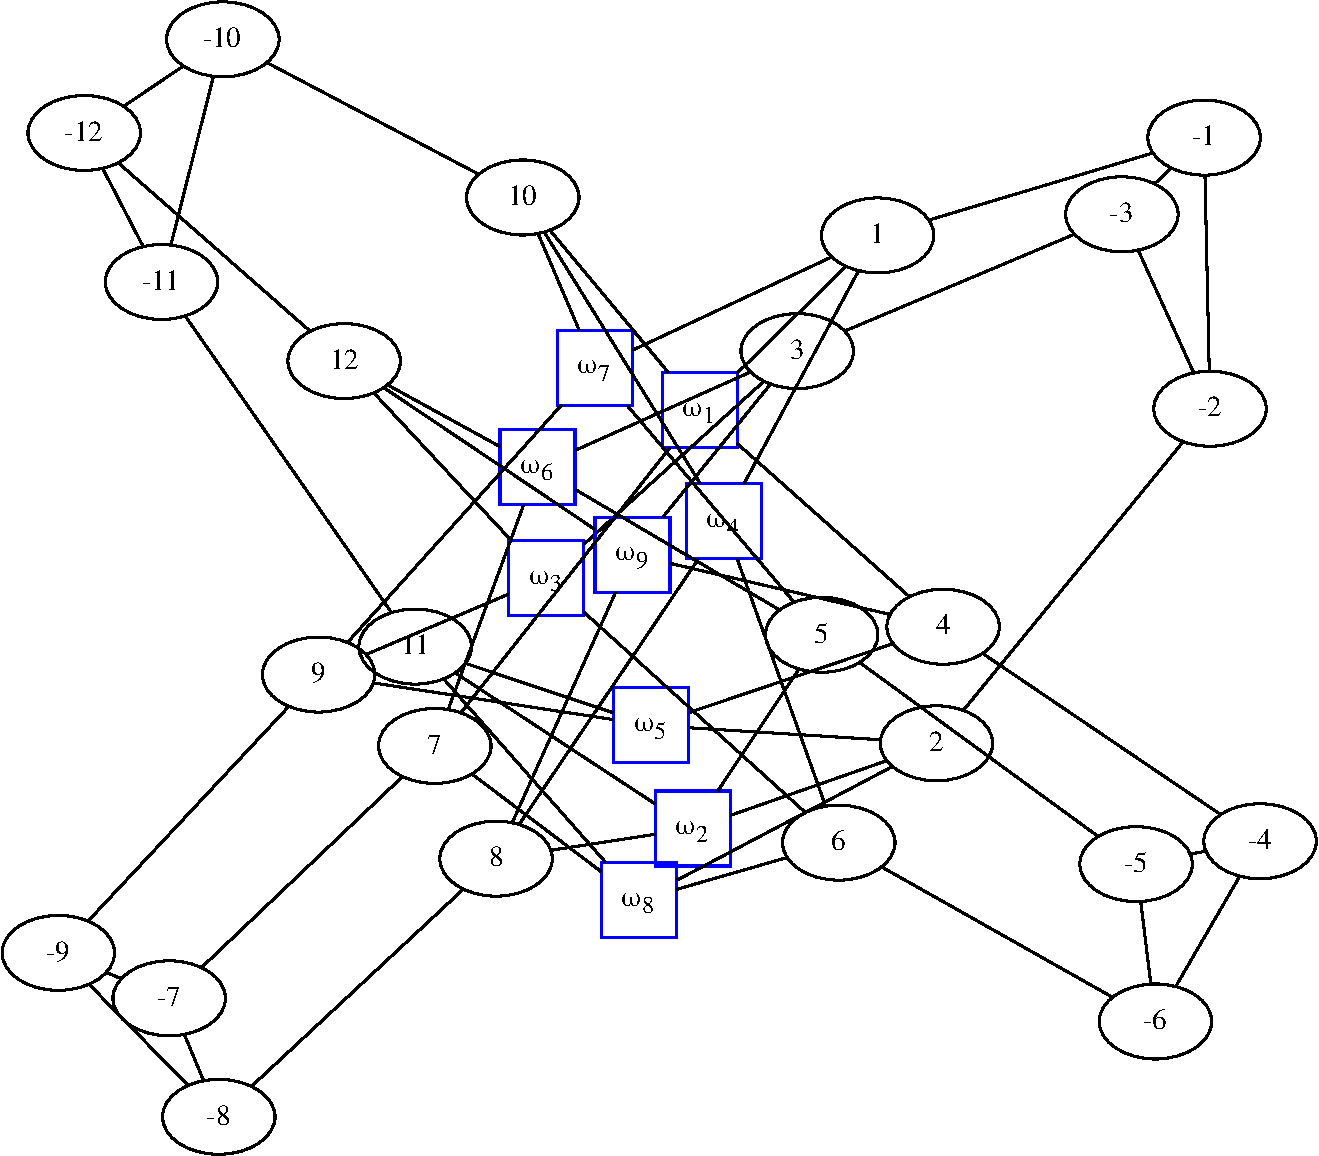
\includegraphics[width=4.3in]{cnfs/graph_cnf_opt-crop}
 \end{minipage}
 \caption{Example of constructed symmetry graph for a given CNF}
  \label{fig:graph_opt}
\end{figure}

After the construction of such a graph, it is given to an automorphism tool which will produce its set of generators.
With the previous graph, the following generators are obtained using $\bliss$ as the automorphism tool:
\begin{center}
 \begin{minipage}[c]{.635\textwidth}
  $g_1 = (x_2 \enskip x_3)(x_5 \enskip x_6)(\neg x_2 \enskip \neg x_3)(\neg x_5 \enskip \neg x_6)$\\
  $g_2 = (x_1 \enskip x_2)(x_4 \enskip x_5)(\neg x_1 \enskip \neg x_2)(\neg x_4 \enskip \neg x_5)$\\
  $g_3 = (x_1 \enskip x_4)(x_2 \enskip x_5)(x_3 \enskip x_6)(\neg x_1 \enskip \neg x_4)(\neg x_2 \enskip \neg x_5)(\neg x_3 \enskip \neg x_6)$
 \end{minipage}
\end{center}
 
\section{Usage of symmetries}

To illustrate the usage of symmetries, consider the \textit{pigeonhole problems} (see \Cref{fig:hole}), where $n$ pigeons are put into $n-1$ holes, with the constraint that each pigeon must be in a different hole. This is a
highly symmetric problem. Indeed, all the pigeons (resp. holes) are exchangeable
without changing the initial problem.
\begin{figure}[!htbp]
 \centering
 \begin{tikzpicture}[
 start chain = going right,
 node distance = 0pt,
 AStyle/.style={draw, minimum width=2em, minimum height=2em, 
  outer sep=0pt, on chain, fill=yellow!0!white}]
 \node [AStyle] (1) {\huge\textcolor{gray}{\PHdove}};
 \node [AStyle] (4) {\huge\textcolor{gray}{\PHdove}};
 \node [AStyle] (5) {\huge\textcolor{gray}{\PHdove}};
 \node [AStyle, draw] (6) {\huge\textcolor{gray}{\PHdove}};
 \node [ minimum width=2em, minimum height=2em, 
 outer sep=1pt, on chain] (7) {\huge\textcolor{gray}{\PHdove}};
 \end{tikzpicture}
 \caption{Graphical representation of an instance of the pigeonhole problem (5 pigeons, 4 holes)}
 \label{fig:hole}
\end{figure}
The search algorithm explores
fruitlessly the symmetric search space, i.e, tries all possible combinations of couples (pigeon, hole).
Solving this problem with a standard SAT solver, like MiniSAT~\cite{een2003extensible},
 turns out to be very time consuming (and even impossible, in a reasonable time, for high values of $n$). 
To avoid this combinatorial explosion, a technique called \emph{symmetry breaking} allows a SAT solver to avoid the visit of symmetric search space. For this purpose, there are two principles , known as \emph{static symmetry breaking}
and \emph{dynamic symmetry breaking}. In the general case, visiting one assignment for each orbit is sufficient to determine the satisfiability of the whole formula.
In the first case, symmetry breaking constraints that invalidate symmetric assignments are added to the initial problem before the start of solving (statically). The second one alters
the search space during the solving (dynamically), it will like in the static approach prune symmetric search space or it can accelerate tree traversal using symmetrical facts.
In fact, some decisions will be transformed into propagations and so accelerate the overall solving time.
  
In the following sections, we present in detail the two principles.

\subsection{Static symmetry breaking}
%Generally symmetry breaking allows SAT solver to avoid the visit of isomorphic search space.
%Visiting one branch is equivalent to visit each symmetric branch and so visiting this one is sufficient to 
%determine satisfiability of the whole formula. Symmetrical branch are discarded by the solver with the addition of 
%constraints. These constraint are not satisfied if the solver visit equivalent assignment.
%In other words, when symmetries of a problems are ignored, solver visit a branch multiple times.
%Consider the \textit{pigeonhole problems} (See \cref{fig:hole}), where $n$ pigeons are put into $n-1$
%holes, with the constraint that each pigeon must be in a different hole is a
%highly symmetric problem. Indeed, all the pigeons (resp. holes) are exchangeable
%without changing the initial problem. Trying to solve it with a standard SAT
%solver, like MiniSAT~\cite{een2003extensible}, turns out to be very time
%consuming (and even impossible, in reasonable time, for high values of $n$).
%Here, such a standard solver ignores the symmetry property of the problem, and
%then potentially tries all variables combinations ; this eventually leads to
%a combinatorial explosion.

This section explains how to statically exploit symmetrical properties of a SAT problem.
In this approach, only one assignment (branch) from each orbit is visited and all others are
omitted.% to deduce the satisfiability of the formula by adding constraints.
This leads us to the following questions:
\begin{enumerate}
 \item How to generate constraints that forbid symmetrical assignments?
 \item How  to choose a branch that is equivalent to all symmetric ones?
\end{enumerate}
To answer question 2, we need to introduce an ordering relation between assignments

\begin{definition}[Assignments ordering]\label{def:assignment_ordering}%
 We assume a total order, $\prec$, on $\Vars$.  Given two assignments $(\alpha,\beta) \in \Assignments(\Vars)^2 $,%
 we say that $\alpha$ is strictly smaller than $\beta$, noted $\alpha < \beta$, if there exists a variable $v \in \Vars$%
 such that:%
 \begin{itemize}%
  \item for all $v' \prec v$, either $v' \in \alpha \cap \beta$ or $\neg v' \in \alpha \cap \beta$.%
  \item $\neg v \in \alpha$ and $v \in \beta$ \footnote{We could have chosen as well $v \in \alpha$ and $\neg v \in \beta$ without loss of generality.}.%
 \end{itemize}%
\end{definition}
In other words, if the prefix of both assignments is equal, according to the ordering relation~$\prec$
and the next variable $v$ has a different value ($\alpha(v) = \false, \beta(v) = \true$), then $\alpha < \beta$.
Note that $<$ coincides with the lexicographical order on \emph{complete}
assignments. 
Furthermore, the $<$ relation is monotonic as expressed by the following proposition:
\begin{proposition}[Monotonicity of assignments ordering]
 \label{prop:monocity_assignments_ordering}
 Let  $(\alpha,\alpha',\beta,\beta') \in \Assignments(\Vars)^4 $ be four assignments.
 $$\text{If}~\alpha \subseteq \alpha'~\text{and}~\beta \subseteq \beta',~\text{then}~\alpha < \beta \implies \alpha' < \beta'$$
\end{proposition}
\begin{proof}
The proposal is a direct result of the definition~\ref{def:assignment_ordering}.
\end{proof}
Given a formula $\varphi$ and its group of symmetries $G$,
the \emph{orbit of $\alpha$ under $G$} (or
simply the \emph{orbit of $\alpha$} when $G$ is clear from the context) is the set
$ [\alpha]_G=\{ g.\alpha \mid g \in G \}$. 
The lexicographic leader (\textit{lex-leader} for short) of an orbit $[\alpha]_G$ is defined by
$min_<([\alpha]_G)$. This \textit{lex-leader} is unique because the lexicographic
order is a total order.
The optimal approach to solve a symmetric SAT problem would be to explore
only one assignment per orbit (for instance each lex-leader).
% \Cref{fig:lex-leader} shows different orbits, each dot in an orbit (ellipse in the figure) is an assignment, and the lex-leader is the empty red one.
%To avoid exploring 
%symmetry search space, \emph{symmetry breaking predicates} (SBP) also called \emph{lex-leader constraints} 
%are added to the formula.
%These constraints are only true for the \emph{lex-leader} \cite{crawford1996symmetry} and prevent other assignments from being explored. 
%\begin{figure}[!htbp]
% \centering
% % \includegraphics[width=2in]{fig/assignment-lex-leader}
% \begin{tikzpicture}
    \tikzstyle{point}=[circle,draw,thick,fill=black,scale=0.2]
	\tikzstyle{point+}=[circle,draw=red,thick,scale=0.4]


\begin{scope}
\node[ellipse, draw, minimum width=4cm, minimum height=2cm] (c1) at (2.5,0){};
	\clip (2.5, 0) ellipse (2 and 1);
	\node[point+] (p2) at (1, 0.3){};
	\pgfmathsetseed{281}
	\foreach \p in {1,...,100}
	{
		\fill (4*rand,2*rand+0.25) circle (0.08);
	}
\end{scope}


\begin{scope}
\node[ellipse, draw, minimum width=4cm, minimum height=2cm] (c1) at (8.5,0){};
\clip (8.5,0) ellipse (2 and 1);
\node[point+] (p2) at (8.6, -0.1){};
\pgfmathsetseed{499478626}
\foreach \p in {1,...,40}
{
	\fill (4*rand+6,2*rand) circle (0.08);
}
\end{scope}

% Legend

\path[draw] (-1, -1.5) -- (13, -1.5);
\node[draw,ellipse, draw, minimum width=4cm, minimum height=2cm, scale=0.1] (ld) at (0, -2) {};
\node[align=left, text width=2.2cm] at (1.5, -2) {Orbit};


\node[circle, fill=black, draw=black, line width=0.5mm, scale=0.3] (lz) at (3, -2) {};
\node[align=left, text width=2.2cm] at (4.5, -2) {Assignment};


\node[point+] (le) at (7, -2) {};
\node[align=left, text width=4.2cm] at (9.5, -2) {Lex-leader assignment};

\path[draw] (-1, -2.7) -- (13, -2.7);



\end{tikzpicture}
% \caption{Show lex-leader per orbit}
% \label{fig:lex-leader}  
%\end{figure}

To answer the first question, the set of lex-leader predicates for a permutation $g \in G_\varphi$ is defined as:
$$LL_g = \forall i : (\forall j < i : x_j = g.x_j) \Rightarrow  x_i \preceq g.x_i$$
In other words, each assignment that has a variable such that its image under $g$ is smaller according to the ordering relation $\prec$, is pruned by $LL_g$.
Conjunction of $LL_g$, for all permutations  $g \in G_{\varphi} $ produces a sound and complete set of symmetry breaking predicates also called \emph{full symmetry breaking}.
In this case, only the lex-leader assignment will be visited for each orbit.
However, the size of the \textit{sbps} can be exponential in the number of variables of the problem and so, they cannot be totally computed.
To overcome this problem, only a subgroup is considered, in this case 
conjunction of $LL_g$ for $H \subset G_{\varphi}$ (such that $g$ is a permutation of the subgroup results a set of symmetry breaking predicates 
that aims at visiting at least one assignment per orbit and is called \emph{partial symmetry breaking}.
In this situation, several assignments per orbit can be visited but often bring a considerable reduction of the
search space. Partial symmetry breaking gives a good trade-off between the number of generated constraints and the reduction of the search space.
In the partial and full symmetry breaking, the set of symmetry breaking predicates generated is denoted by $\psi$.
%\hakan{A REVOIR}
%Since  a group may have an exponential number of permutations, all symmetry breaking predicates belong
%to the group must be generated to ensure full symmetry breaking. These constraints will overload the 
%solver and slow down its core principle (unit propagation). Hence, slow down overall time computation.
%Conversely, partial symmetry breaking adds few constraints and bring often considerable reduction of the
%search space. Generally, the set of generators produced by automorphism tool is chosen as a subgroup.
%Partial symmetry breaking gives a good trade off between the number of generated constraints and reduction of the search space.
%
%To ensure the visiting only the lex leader, all SBPs of all permutations 
%belongs to the group must be generated.
%Adding too many SBPs clauses will overload the solver and slow down the unit propagation.
%
%When only one assignment per orbit (generally the lex-leader) is visited, this is called  \emph{full symmetry breaking}.
%Conversely, \emph{partial symmetry breaking} aims to visit at least one assignment per orbit.
%Only some of the permutations are used to generate SBPS, that are generally  the set of generators 
%given by the automorphism tool.
%This approach is more easy to set up and bring considerable reduction of the search spaces.
%in some $G \subseteq G_{\varphi} $ results a sound and complete symmetry breaking predicates
%but not necessarily \emph{complete} symmetry breaking predicates for $G_{\varphi}$ noted $\psi$.

\begin{theorem}[Satisfiability preservation SBPs]
 \label{theorem:satisfiability_preservation_SBPs}
 Let $\varphi$ be a formula and $\psi$ the computed \textit{SBPs} for the set of symmetries in $G_{\varphi}$: 
 $$\varphi~and ~\varphi \wedge \psi \text{ are equi-satisfiable}.$$
\end{theorem}

\begin{proof}
 If $\varphi \wedge \psi$ is SAT then $\varphi$ is trivially SAT. If
 $\varphi$ is SAT, then there is some assignment $\beta$ that satisfies $\varphi$.
 Without loss of generality, $\beta$ can be chosen to be the lex-leader of its
 orbit under $G_{\varphi}$. Thus, $g$ does not contradict $\beta$, which implies that
 $\beta \models \psi$.
\end{proof}

% By definition of an orbit, it exists a permutation that map each assignment to another in the same orbit. 
%
%Lex-leader constraints are build for each permutation in the group.
%Given a permutation 
%Generation of these lex-leaders constraints proposed by Crawford et al.~\cite{crawford1996symmetry}:
%
%$$\forall i : (\forall j < i : x_j = g.x_j) \Rightarrow  x_i \preceq g.x_i$$
%
%In other words, assuming the ordering relation depicted in \Cref{def:assignment_ordering}, for one permutation,
%these constraint express that the value of the variable $x_i$ must be smaller or equal than the
%value of $g.x_i$ and all variables $x_j$ that respect the constraint $x_j \prec x_i$,  
%must have the same value of its symmetric. As such, these constraints encodes a valid 
%lex leader with respect to this permutation.
The generation of lex-leader constraints proposed by Crawford et al.~\cite{crawford1996symmetry} is defined as follows:
$$ LL_g = \forall i : (\forall j < i : x_j = g.x_j) \Rightarrow  \neg x_i \lor g.x_i$$
 
 \Cref{fig:esbp_gen} shows an example of the generated clauses for the  permutation $g_3$ of the previous 
 example and a lexicographic order. The last constraint of the figure produces tautological clauses.
 Actually variables $x_1$, $x_4$ are present with both polarities. The constraints of other variables also produce 
 tautological clauses. 
 
 \begin{figure}[!htbp]
  
total order $ x_1 \prec x_2 \prec x_3 \prec x_4 \prec x_5 \prec x_6$\\
permutation $g_1 = (x_2 \enskip x_3)(x_5 \enskip x_6)(\neg x_2 \enskip \neg x_3)(\neg x_5 \enskip \neg x_6)$\\


$x_2 \preceq x_3$ \\
$x_2 = x_3 \implies x_5 \preceq x_6$\\

%2 == 3 -> 3 <= 2
%2 == 3 \land 3 == 2 -> 5 <= 6
  \caption{Example of generated SBPs for one permutation}
  \label{fig:esbp_gen}
 \end{figure}
Here, the number of clauses generated per constraint increase exponentially by the 
cardinality of the support  of the permutation. Hence, Aloul et al~\cite{aloul06} proposed a more compact representation of \textit{sbps} based on the creation of auxiliary variables.  
These variables encode equality of literals and are disjoint from the support of the permutation.
Following clauses encode a compact lex-leader for a permutation:
%Let $g$ for a permutation, let $\support_g$ = $\{x_1, \cdots, x_n\}$ the support of $g$ be ordered 
% such that $x_i \preceq x_j$ iff $i \leq j$  and let $\{y_0,\cdots, y_{n} \}$ be a set of auxiliary variables
% disjoint from $\support_g$. These auxiliary variables encode equality of literals in such $y_0$ is set as an unit clause
% and encodes the first equality.
 
\begin{center}
\begin{tabular}{cc|cc}
 $\neg y_i \lor \neg x_{i-1} \lor \neg x_i \lor g.x_i$ & $1 \leq i \leq n$ & $ \neg y_i \lor \neg x_{i-1} \lor y_{i+1}$ & $1 \leq i \leq n$ \\
 $\neg y_i \lor  g.x_{i-1} \lor \neg x_i \lor g.x_i$ & $1 \leq i \leq n$ & $ \neg y_i \lor g.x_{i-1} \lor  y_{i+1}$ & $1 \leq i \leq n$ \\
 
\end{tabular}
\end{center}
where $\{y_0,\cdots, y_{n} \}$ is the set of auxiliary variables, $y_0$ is a unit clause that encodes the first equality and $\{x_1,...,x_n\}$ be the set of variables sorted with the lexicographic order.

\Cref{fig:esbp_compact_gen} shows the compact encoding of generated constraints. This form grows linearly w.r.t. the number of variables.
The auxiliary variables that encode the equality of two literals provide this reduction. 
Three auxiliary variables are introduced in this example $x_7,\ x_8,\ x_9$ such that $x_7$ encodes the equality of $x_1$ and $x_4$, $x_8$ encodes the equality of $x_2$ and $x_5$, and $x_9$ encodes the equality of $x_3$ and $x_6$.
 \begin{figure}[!htbp]
 


\begin{center}
	\begin{tabular}{lll}
		Order &:& $ x_1 \prec x_2 \prec x_3 \prec x_4 \prec x_5 \prec x_6 \enskip ; \enskip  (\false < \true)$ \\
		Permutation &:& $g_3 = (x_1 \enskip x_4)(x_2 \enskip x_5)(x_3 \enskip x_6)(\neg x_1 \enskip \neg x_4)(\neg x_2 \enskip \neg x_5)(\neg x_3 \enskip \neg x_6)$
	\end{tabular}
	
	\vspace*{2\baselineskip}
	
	\begin{tabular}{ll}
		Constraints & Generated SBP\\
		\midrule
		$x_1 \preceq x_4$ & $ \neg x_1 \lor x_4$ \\
		& $x_7$ \\
		&\\
		$x_1 = x_4 \Rightarrow x_2 \preceq x_5$ &  $ \neg x_7 \lor \neg x_1 \lor \neg x_2 \lor x_5$\\
		& $ \neg x_7 \lor \neg x_1 \lor x_8$\\
		& $ \neg x_7 \lor  x_4 \lor \neg x_2 \lor x_5$ \\
		& $ \neg x_7 \lor x_4 \lor x_8$\\
		
		&\\
		$x_1 = x_4 \land x_2 = x_5 \Rightarrow x_3 \preceq x_6$ 
		& $\neg x_8 \lor \neg x_2 \lor \neg x_3 \lor x_6$\\
		& $\neg x_8 \lor \neg x_2 \lor x_9$\\
		& $\neg x_8 \lor x_5 \lor \neg x_3 \lor x_6$\\
		& $\neg x_8 \lor x_5 \lor x_9$\\

	\end{tabular}
\end{center}
 \caption{Example of compact generated SBPs for one permutation}
 \label{fig:esbp_compact_gen}
\end{figure}
$\shatter$ is a tool~\cite{aloul06} for partial symmetry breaking.
It computes a compact lex-leader \textit{sbps} with the symmetries produced by $\saucy$~\cite{katebi2010symmetry}.
The following table shows the number of symmetry breaking predicates and the
number of auxiliary variables added to the original formula.

\begin{center}
	\hakan{Mette des espaces pour les nombres et texte pour expliquer si tableau ok}\\
	\hakan{Mettre total de clause et vars et pourcentage d'augmentation}
\begin{tabular}{lcccc}
	Instances & \#vars & \#clause & \#sbp & \#auxiliary variables \\
	\toprule
	\detokenize{battleship-12-12-unsat} &  936 &  144 &  1498 &  378\\
	\detokenize{battleship-12-23-sat} &  1662 &  276 &  5464 &  1375\\
	\detokenize{battleship-14-26-sat} &  2562 &  364 &  3688 &  929\\
	\detokenize{battleship-14-27-sat} &  2653 &  378 &  7222 &  1814\\
	\detokenize{battleship-16-16-unsat} &  2176 &  256 &  4388 &  1102\\
	\detokenize{battleship-16-31-sat} &  3976 &  496 &  12094 &  3035\\
	\detokenize{battleship-24-57-sat} &  16308 &  1368 &  40372 &  10113\\
	\midrule
	\detokenize{chnl10_11} &  1122 &  220 &  2416 &  615\\
	\detokenize{chnl10_12} &  1344 &  240 &  2736 &  696\\
	\detokenize{chnl10_13} &  1586 &  260 &  3252 &  826\\
	\detokenize{chnl11_12} &  1476 &  264 &  3204 &  813\\
	\detokenize{chnl11_13} &  1742 &  286 &  3636 &  922\\
	\detokenize{chnl11_20} &  4220 &  440 &  6760 &  1710\\
	\midrule
	\detokenize{fpga10_15_uns_rcr} &  2130 &  300 &  4580 &  1160\\
	\detokenize{fpga10_20_uns_rcr} &  3840 &  400 &  6768 &  1712\\
	\detokenize{fpga11_12_uns_rcr} &  1476 &  264 &  3704 &  938\\
	\detokenize{fpga11_13_uns_rcr} &  1742 &  286 &  4076 &  1032\\
	\detokenize{fpga11_14_uns_rcr} &  2030 &  308 &  4740 &  1199\\
	\detokenize{fpga11_15_uns_rcr} &  2340 &  330 &  5196 &  1314\\
	\detokenize{fpga11_20_uns_rcr} &  4220 &  440 &  7864 &  1986\\
	\midrule
	\detokenize{hole010} &  561 &  110 &  1054 &  269\\
	\detokenize{hole015} &  1816 &  240 &  3280 &  828\\
	\detokenize{hole020} &  4221 &  420 &  6478 &  1630\\
	\detokenize{hole030} &  13981 &  930 &  21322 &  5346\\
	\detokenize{hole040} &  32841 &  1640 &  44934 &  11254\\
	\detokenize{hole050} &  63801 &  2550 &  81682 &  20446\\
	\midrule
	\detokenize{Urq6_5} &  1756 &  180 &  109 &  0\\
	\detokenize{Urq7_5} &  2194 &  240 &  143 &  0\\
	\detokenize{Urq8_5} &  3252 &  327 &  200 &  0\\
	\midrule
	\detokenize{x1_40} &  314 &  118 &  42 &  1\\
	\detokenize{x1_80} &  634 &  238 &  80 &  0\\
\end{tabular}
\end{center}

\Cref{tab:numsbp} presents the number of variables and clauses present in the formula and also the  
number of \textit{sbps} generated and the number of auxiliary variables added on different problem categories that are:
battleship (the battleship puzzle), chnl (channel routing instances), fpga (routing of global wires in integrated circuits),
 hole (the pigeonhole problem), urq (randomized instance based on expanded graphs), xor (exclusive or chain).\\
We can observe that the number of produced \textit{sbps} and added auxiliary variables can be much larger than
respectively the number of initial clauses and variables.

%\hakan{mettre tableauw nombre de SBP generé}
%
%\begin{figure}[!htbp]
% \centering
% \includegraphics[height=5cm]{example-image-a}
% \label{}
%\end{figure}
%An improvement of static symmetry breaking was made by Devriendt et al~\cite{devriendt2016improved} with a tool 
%called $\breakid$. It exploits some properties from the structure of the generators. On some cases, 
%a linear number of constraints can break all group. It also tries to add a maximum of binary clauses.
%These can accelerate the unit propagation and participate to the conflict analysis.
\subsubsection{Special form of the group} \label{sec:matrix-sbp}
Some formulas exhibit a specific type of symmetry, called \emph{row (column) interchangeability}. These are
a subset of variables structured as a two-dimensional matrix. Each row (column) is interchangeable,
so, all variables of a row (column) permute with any other one.
This form of symmetry is common in different kinds of problems like the pigeon hole problem in which
pigeons and holes are interchangeable. % or in the delivery system in which trucks of a fleet are interchangeables.
The usage of row (column) interchangeability can significantly improve SAT performance. 
Actual symmetries can be eliminated by the addition 
of only a linear number of symmetry-breaking constraints~\cite{flener2002breaking}. 
To ensure this linear number of constraints, one condition must be satisfied :
the lexicographic order of variables needs to respect the structure of the matrix.
In practice, automorphism tools give only  set of generators that contains no information on
the structure of the group. 
The authors of $\breakid$~\cite{devriendt2016improved} developed an algorithm to detect this specific 
structure and exploit it.
%Another improvement made by $\breakid$ is the exploitation of binary constraints
%An improvement of static symmetry breaking was made by Devriendt et al~\cite{devriendt2016improved} with a tool 
%called $\breakid$. It exploits some properties from the structure of the generators. On some cases, 
%a linear number of constraints allows to visit only one assignment for each orbit.
% It also tries to add a maximum of binary clauses.
% These can accelerate the unit propagation and participate to the conflict analysis.
\subsubsection{Binary lex-leader constraints}
$\breakid$ tries to generate a maximum number of binary lex-leader constraints.
The first lex-leader constraint generated by each permutation is a binary clause.
Enumerating the whole symmetry group will generate many binary clauses but will be time consuming.
To avoid this enumeration, the  graph structure  of the orbit is exploited: as the orbit can be seen as a strongly connected component, there must exist a permutation that permutes a variable (for example the smallest variable according to the lexicographic order) of an orbit with each of the other variables of the same orbit. This allows us to
generate as many binary lex-leader constraints as the size of the orbit. In addition, constructing 
a sequence of subgroups that stabilize the smallest variable allows the generation of new binary \textit{sbps}.
This sequence ends when a trivial subgroup is reached and is called a  \emph{stabilizer chain}.
\Cref{fig:binary_sbp} shows the application of the stabilizer chain.
In the example, the considered group has three permutations and its graphical representation
is shown. Given the lexicographic order, the smallest variable is $x_1$ and 
all other variables are in its orbit. According to the ordering relation, five 
\textit{sbps} are generated, one \textit{sbp} for each variable of the orbit except the smallest one.
Then, the subgroup that stabilizes $x_1$ is computed. It contains only one permutation $(g_2)$.
As $x_2$ is the smallest variable according to the lexicographic order, the constraint $\neg x_2 \lor x_3$ is generated. The stabilizer chain leads to a trivial group and no more binary clauses are generated.
In total, six binary clauses are generated without adding any auxiliary variables.
Moreover, a property can be observed, when the smallest variable has the greatest value 
($\true$ in this case), all variables in the orbits must have the same value.
 \begin{figure}[!htbp]
 
\begin{center}
\begin{tabular}{lll}
	Order &:& $ x_1 \prec x_2 \prec x_3 \prec x_4 \prec x_5 \prec x_6 \enskip \mid \enskip  (\false < \true)$ \\
\end{tabular}
\end{center}
\vspace*{1\baselineskip}
	
\begin{minipage}[c]{.635\textwidth}
	\footnotesize
	$\textcolor{green_1}{g_1 = (x_2 \enskip x_3)(x_5 \enskip x_6)(\neg x_2 \enskip \neg x_3)(\neg x_5 \enskip \neg x_6)}$\\
	$\textcolor{blue_1}{g_2 = (x_1 \enskip x_2)(x_4 \enskip x_5)(\neg x_1 \enskip \neg x_2)(\neg x_4 \enskip \neg x_5)}$\\
	$\textcolor{red_1}{g_3 = (x_1 \enskip x_4)(x_2 \enskip x_5)(x_3 \enskip x_6)(\neg x_1 \enskip \neg x_4)(\neg x_2 \enskip \neg x_5)(\neg x_3 \enskip \neg x_6)}$

	\vspace*{2\baselineskip}
	
\begin{tikzpicture}[level/.style={sibling distance=60mm/#1},every node/.style={scale=0.6}, scale=0.6]
	\tikzstyle{orbit-node}=[draw,circle,minimum size=35pt,inner sep=0pt]
	\tikzstyle{g1}=[->, draw, color=blue_1, line width=1pt]
	\tikzstyle{g2}=[->, draw, color=green_1, line width=1pt]
	\tikzstyle{g3}=[->, draw, color=red_1, line width=1pt]
	
	\tikzstyle{g}=[->, draw, color=black, line width=1pt]
		
	\node[orbit-node, fill=orange!30] (1) {$x_1$};
	\node[orbit-node] (2) at ($(1) + (5, 0)$) {$x_2$};
	\node[orbit-node] (3) at ($(2) + (5, 0)$) {$x_3$};
	\node[orbit-node] (4) at ($(1) + (0, -4)$) {$x_4$};
	\node[orbit-node] (5) at ($(1) + (5, -4)$) {$x_5$};
	\node[orbit-node] (6) at ($(2) + (5, -4)$) {$x_6$};
	
	% g1
	\draw[g1] (1) to [bend right=10] (2);
	\draw[g1] (2) to [bend right=10] (1);
	
	\draw[g1] (4) to [bend right=10] (5);
	\draw[g1] (5) to [bend right=10] (4);
	
	
	%g2
	
	\draw[g2] (2) to [bend right=10] (3);
	\draw[g2] (3) to [bend right=10] (2);
	
	\draw[g2] (5) to [bend right=10] (6);
	\draw[g2] (6) to [bend right=10] (5);
	
	% g3
	\draw[g3] (1) to [bend right=10] (4);
	\draw[g3] (4) to [bend right=10] (1);
	
	\draw[g3] (2) to [bend right=10] (5);
	\draw[g3] (5) to [bend right=10] (2);
	
	\draw[g3] (3) to [bend right=10] (6);
	\draw[g3] (6) to [bend right=10] (3);
	
	\draw[g] (1) to [bend left=25] (3);
	\draw[g] (1) to [] (5);
	\draw[g] (1) to [bend left=0] (6);
\end{tikzpicture}
\end{minipage}
\begin{minipage}[c]{.635\textwidth}
	\footnotesize
	$\textcolor{green_1}{g_1 = (x_2 \enskip x_3)(x_5 \enskip x_6)(\neg x_2 \enskip \neg x_3)(\neg x_5 \enskip \neg x_6)}$\\
	
	\vspace*{4.5\baselineskip}
	
	\begin{tikzpicture}[level/.style={sibling distance=60mm/#1},every node/.style={scale=0.6}, scale=0.6]
	\tikzstyle{orbit-node}=[draw,circle,minimum size=35pt,inner sep=0pt]
	\tikzstyle{g1}=[->, draw, color=blue_1, line width=1pt]
	\tikzstyle{g2}=[->, draw, color=green_1, line width=1pt]
	\tikzstyle{g3}=[->, draw, color=red_1, line width=1pt]
	
	\tikzstyle{g}=[->, draw, color=black, line width=1pt]
	
	\node[orbit-node,fill=orange!30] (2) {$x_2$};
	\node[orbit-node] (3) at ($(1) + (5, 0)$) {$x_3$};

	\node[orbit-node] (5) at ($(1) + (0, -4)$) {$x_5$};
	\node[orbit-node] (6) at ($(1) + (5, -4)$) {$x_6$};

	\draw[g2] (2) to [bend right=10] (3);
	\draw[g2] (3) to [bend right=10] (2);
	
	\draw[g2] (5) to [bend right=10] (6);
	\draw[g2] (6) to [bend right=10] (5);
	
	\end{tikzpicture}
\end{minipage}

\vspace*{1\baselineskip}

\begin{minipage}[l]{.58\textwidth}
	\begin{itemize}
		\item[] $\omega_{1} = \{\neg x_1, x_2\}$\hspace*{2em} $\omega_{4} = \{\neg x_1, x_5\}$
		\item[] $\omega_{2} = \{\neg x_1, x_3\}$\hspace*{2em} $\omega_{5} = \{\neg x_1, x_6\}$
		\item[] $\omega_{3} = \{\neg x_1, x_4\}$
	\end{itemize}
\end{minipage}
\begin{minipage}[l]{.635\textwidth}
	\begin{itemize}
		\item[] $\omega_{6} = \{\neg x_2, x_3\}$
	\end{itemize}
\end{minipage}
 \caption{Generation of binary symmetry breaking predicates}
 \label{fig:binary_sbp}
\end{figure}
The size of the stabilizer chain is heavily dependent on the chosen lexicographic order.
To avoid reaching trivial subgroups quickly an incremental order is proposed.
%to optimize the number of generates binary clauses. 
It uses the size of the orbit and occurrences of variables in the set of generators:
the biggest orbit produces more binary clauses and variables with few occurrences allow to disable less generators.

\subsubsection{BreakID}
As summary, $\breakid$ combines three ideas:i) It searches if produced the generators by the automorphism tool 
have the row interchangeability special form and exploit;
ii) It generates a maximum number of binary lex-leader constraints; iii) The classical \textit{sbps} are 
generated.

%The exploitation of symmetries statically is called \emph{static symmetry breaking}.
%It acts like a preprocessor which add \emph{symmetry breaking predicates} (SBPs) at the 
%original formula and solve the augmented problem. 
%This approach gives good performances in practice.
%
%\hakan{Conclu static}

\subsubsection{Conclusion}
Static symmetry breaking approach acts as a preprocessor that augment the initial formula with
\textit{sbps}. These constraints avoid the exploration of isomorphic search spaces.
In the general case, the number of these clauses is often too large to be
 handled  effectively by a SAT solver~\cite{Luks2004}. 
On the other hand, if only a subset of the symmetries is considered then the resulting search pruning
will not be perfect and its effectiveness will depend heavily on the symmetries chosen heuristically. 
 \cite{biere2009handbook}.
An important point in static symmetry breaking is the chosen lexicographic order.
Variable ordering may impact the number of generated constraints and hence the performance of
the underlying solver. Different orders are studied in the literature. 
One of the simplest order is the  lexicographical order.
Some other existing orders exploit the structural properties of the 
problem~\cite{devriendt2016improved}. Combining the generation of binary \textit{sbps} with the exploitation of
these properties allows state-of-the-art solver to solve more symmetric instances.
Despite these optimizations and the good reduction of the search space with symmetries,
some formula that exhibit symmetries are still intractable for a state-of-the-art SAT solver.
%In the general case, the size of the \textit{sbps} can be exponential in the number of variables of
%the problem so that they cannot be totally computed. Even in  favorable
%situations, the size of the generated \textit{sbps} is often too large to be
%effectively handled by a SAT solver~\cite{luks.04.amai}. On the other hand, if
%only a subset of the symmetries is considered then the resulting search pruning
%will not be that interesting and its effectiveness depends heavily on the
%heuristically chosen symmetries \cite{biere2009handbook}. 
Moreover, a disadvantage of static symmetry breaking is that the solver is influenced by \textit{sbps}.
Internal heuristics consider these clauses as the original clauses, so the solver explores
the search space with a different manner and affects performance negatively.

%
%Besides, these approaches
%are preprocessors, so their combination with other techniques, such as
%\emph{symmetry propagation}~\cite{Devriendt12}, can be very hard.
%
%Also, tuning their parameters during the solving turns out to be very difficult. For all
%these reasons, some classes of SAT problems cannot be solved yet despite
%exhibiting symmetries.
%
%
%Actually, the number of generates sbps can slow down the solver core mechanism (unit propagation) 

%\begin{figure}[!htbp]
%   \newcolumntype{C}{ >{\centering\arraybackslash} m{8cm} }
  \newcolumntype{D}{ >{\centering\arraybackslash} m{6cm} }
  \begin{tabular}{DC}
    CNF\ formula &{\scriptsize
          \begin{tabular}{c}
          	$ \{ x_{1}, x_{2}, x_{3} \}$,
          	$ \{ x_{4}, x_{5}, x_{6} \}$,
          	$ \{ x_{1}, x_{4} \}$ \\
          	$ \{ x_{2}, x_{5} \}$,
          	$ \{ x_{3}, x_{6} \}$ ,
          	$ \{ \neg x_{1}, \neg x_{2} \}$ \\
          	$ \{ \neg x_{1}, \neg x_{3} \}$,
          	$ \{ \neg x_{2}, \neg x_{3} \}$,
          	$ \{ \neg x_{4}, \neg x_{5} \}$\\
          	$ \{ \neg x_{4}, \neg x_{6} \}$,
          	$ \{ \neg x_{5}, \neg x_{6} \}$            
          \end{tabular}}\\
      & \\
    $\Downarrow$ & $\Downarrow$  \\
          & \\
    colored graph & 		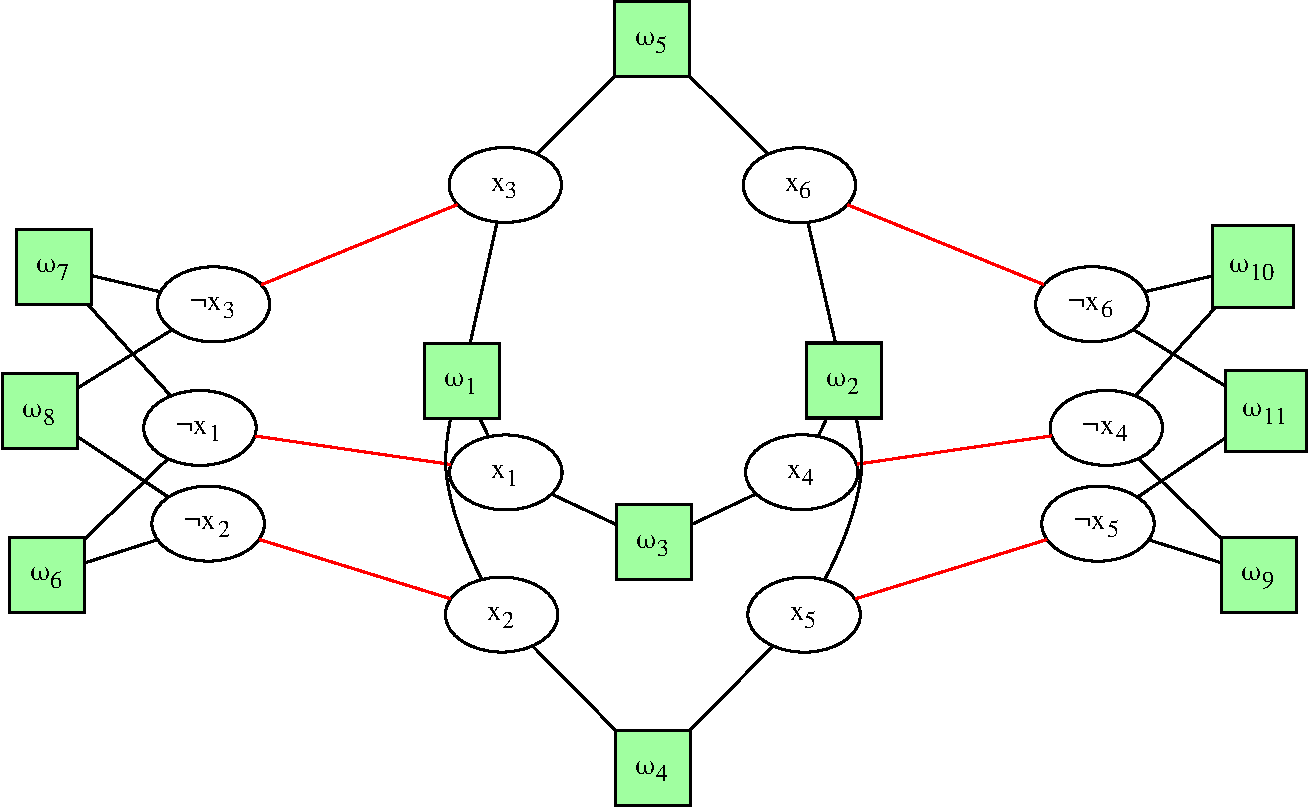
\includegraphics[width=2.5in]{cnfs/graph_cnf_no_opt-crop}\\

    $\|$ & $\|$  \\
        & \\
    graph automorphism &
                         \small{(\texttt{bliss} \footnote{http://www.tcs.hut.fi/Software/bliss/} or
                         \texttt{saucy} \footnote{http://vlsicad.eecs.umich.edu/BK/SAUCY/})}
    \\
  
        & \\
    $\Downarrow$ & $\Downarrow$  \\
      & \\
    set of symmetries & \begin{minipage}[l]{\textheight}
    	\footnotesize
    	$g_1 = (x_2 \enskip x_3)(x_5 \enskip x_6)(\neg x_2 \enskip \neg x_3)(\neg x_5 \enskip \neg x_6)$\\
    	$g_2 = (x_1 \enskip x_2)(x_4 \enskip x_5)(\neg x_1 \enskip \neg x_2)(\neg x_4 \enskip \neg x_5)$\\
    	$g_3 = (x_1 \enskip x_4)(x_2 \enskip x_5)(x_3 \enskip x_6)(\neg x_1 \enskip \neg x_4)(\neg x_2 \enskip \neg x_5)(\neg x_3 \enskip \neg x_6)$
    \end{minipage}  \\
  \end{tabular}
% \caption{Caption}
% \label{fig:big_picture_static}
%\end{figure}

\subsection{Dynamic symmetry breaking}

Dynamic symmetry breaking approaches aims at exploiting the symmetries during the solving by altering the behavior of the solver.
During the solving, the solver uses symmetries (present in the formula) to remove symmetric assignments or to propagate symmetrical facts.
Propagating symmetrical facts has the consequence of reducing the number of decisions that are chosen heuristically and increase the number of propagations.
In other words, symmetries transform some “guesses” into “deductions”. So, it improves the performance of the underlying solver.
In the literature, different approaches of dynamic symmetry breaking exist, this section presents the most important of them.

\subsubsection{SymChaff}
One of the first tools for dynamic symmetry breaking is \emph{SymChaff} a structure-aware SAT solver~\cite{sabharwal2005symchaff}
and applies only on particular groups (\cref{sec:matrix-sbp}).
To take part of this property, instead of using the classical decision heuristic that chooses exactly one
variable, all symmetric variables are considered at the same time (k-branching). 
Roughly speaking, all variable in the same orbit are assigned/unassigned at the same time. So, all possible valuation 
of the orbit can be checked once. In this approach, only the number of true and false literal matters
and computing the number of possible valuations is trivial in this particular 
form of group. For example, consider the permutations: $g_1 = (1\, 2)$,
only one of the valuations $F T$ (variable $1$ assigned to the false value and variable $2$ assigned to the true value) or the reverse assignment ($T F$).
 So, one true value and one false value must be checked in addition to the 
$F F$ and $T T$ assignments to determine the satisfiability of the formula.
 The order in which the valuations are checked has a tremendous impact on solver performance. 
This approach has good results when the group of symmetries presents a particular form.
In the general case, when we consider any group, computing the number of possible valuation will be very difficult and this approach is not applicable.

\subsubsection{Symmetry Propagation}
A different approach can be used to accelerate the tree traversal using symmetrical facts during the solving.
One of them is \emph{symmetry propagation} (SP)~\cite{Devriendt12}.
The general idea of this approach is to propagate symmetrical literals of those already propagated.
In other words, it accelerates the tree traversal by ``transforming some guess (decisions) to deductions (propagations)''.
%Indeed, the problem that presents symmetries makes possible to deduce some value 
%for the variables that would be guessed if symmetry properties were ignored.
These deductions will reduce the overall tree traversal depth and hence will eventually accelerate the solving process. To explain this approach, 
let first give some definitions.
\begin{definition}[Logical consequence]
 \label{def:logical_consequence}
 A formula $\phi$ is a logical consequence of a formula $\varphi$ denoted by $\varphi \models \phi$, if for any assignment
 $\alpha$ satisfying $\varphi$, also satisfies $\phi$. Two formulas are \emph{logically equivalent} if each is a logical
 consequence of the other.
\end{definition}
\begin{proposition}[Symmetry propagation]
 \label{prop:symmetry_propagation}
 Let $\varphi$ be a formula, $\alpha$ an assignment and $l$ a literal. 
 If $g$ is a symmetry (permutation) of $\varphi \cup \alpha$ and
 $\varphi \models \{l\}$, then $\varphi \cup \alpha \models g.\{l\}$.
\end{proposition}
In other words, if a literal $l$ is propagated by the solver and $g$ is a \emph{valid} symmetry for the
sub problem $\varphi \cup \alpha$ (in which all satisfied clauses and false literals are removed) then, the solver can
also propagate the symmetric of $l$. The problem here is to determinate which symmetries are valid for the formula
$\varphi \cup \alpha$.
\begin{definition}[Active symmetry]
 \label{def:active_symmetry}
 A symmetry $g$ is called active under a partial assignment $\alpha$ $\text{if } g.\alpha = \alpha$
\end{definition}
Definition~\ref{def:active_symmetry} leads to the following proposition:
\begin{proposition}
 \label{prop:active_symmetry}
 Let $\varphi$ a formula and $\alpha$ a partial assignment. Let $g$ be a symmetry of $\varphi$,
 if $g$ is active under the assignment $\alpha$, then $g$ is also a symmetry of $\varphi \cup \alpha$.
\end{proposition}
The previous proposition states that an active symmetry $g$ for a partial assignment $\alpha$ is still valid for
the formula $\varphi \cup \alpha$. So when a literal $l$ is propagated, and a symmetry $g$ is active for a
partial assignment $\alpha$, the solver can also propagate $g.l$. 
Moreover, the group theory allows to compose permutations, and the composition of two active symmetries is also an active symmetry,
so the solver can also propagate. $g^2.l, g^3.l, ... $

Active symmetries need strong requirements and so their applications are limited.
Devriendt et al~\cite{Devriendt12} improved the notion of active symmetries in the SAT context by
introducing the notion \emph{weakly active} symmetries that relax some constraints.
%\hakan{revoir def avec soheib}
\begin{definition}[Weakly active symmetry]
 \label{def:weakly_active_symmetry}
 Let $\varphi$ be a formula and ($\delta, \alpha, \gamma$) a state of a CDCL solver in which $\delta$ is the set of decisions
 $\alpha$ is the current assignment and $\gamma$ the reasons of the learned clauses. Then a symmetry $g$ is weakly active 
 if $g.\delta \subseteq \alpha$
\end{definition}
This definition leads to the following proposition:
\begin{proposition}
 Let $\varphi$ be a formula, $\alpha $ an assignment. If
 there exists a subset $\delta \subseteq \alpha $ and a symmetry $g$ of $\varphi$ such that 
 $g.\delta \subseteq \alpha $ and $\varphi \cup \delta \models \varphi \cup \alpha$, then $g$ 
 also is a symmetry of $\varphi \cup \alpha $.
\end{proposition}

In other words, we can detect with minimal effort the symmetries of $\varphi
\cup \alpha$ by keeping track of the set of variables $\delta$, which are 
in state-of-the-art complete SAT solving algorithms, the set of decision variables.
Obviously, a weakly active symmetry can also propagate the symmetrical literals of a propagated one.
Moreover, weakly active symmetries allow more propagations and so are more efficient.
%Note that if a weakly active symmetry wants to propagate a symmetrical literal which are already affected to the 
%opposite value, this leads to a symmetry conflict and the solver backtrack to propagate the symmetrical value correctly.
%\hakan{Mettre des tableaux, courbes etc ...}\\
%\hakan{Courbe VS static an no sbp}\\
%\hakan{Conclu SP, depend on the solver choice}\\
Symmetry propagation gives good performances on many symmetric instances.
The overall performance of the symmetry propagation is intrinsically related to the decision heuristics of the underlying SAT solver.
%In addition, this approach don't discard any assignments like in the static approaches where 
%non lex-leader assignments are eliminated.
%One optimization of symmetry propagation is the following proposition, as seen in 
% each propagated clause has a reason which is an assertive clause.
%If the symmetrical clause is also an assertive one, this clause can be added in the formula without any requirements
%(even if the permutation is not weakly active). The added symmetrical clause will also participate to unit propagation and propagate the symmetrical literal.
\subsubsection{Symmetry Explanation Learning}

Another approach to exploit symmetry without removing any satisfiable assignment of the problem
is \emph{Symmetry Explanation Learning}~\cite{devriendt2017symmetric} (SEL). 
Symmetries of a formula leave this last invariant. Moreover, all learned clauses are logical consequences of the problem, symmetric of these clauses are also valid.
Unlike Symmetry explanation scheme~\cite{benhamou2010enhancing} (SLS) where all symmetrical learned clauses
are added to the clause database.
The idea of this approach is to learn useful symmetrical variants of learnt clauses.
 A clause is said to be useful if it participates to the unit propagation or conflict analysis.
Computing all symmetrical learnt clauses will create a huge overhead in terms of computation time and memory.
Its usage will be limited on huge problems.
% As symmetries leave the formula, the symmetrical clauses can be already
%in managed clause by the solver and make unit propagation heavier.
To avoid the previous drawback, SEL uses the following fact:
i) All modern CDCL solvers need to maintain the implication graph and so store the reason of the propagated literals and
obviously this reason is assertive.
ii) Symmetries permute only few literals in a clause and so the probability that symmetrical clauses are also assertive is high.
So, symmetrical clauses may also participate to the unit propagation.
iii) These clauses are stored in different learning database and 
treated separately. The solver promotes these clauses when they are effectively useful
at the end of unit propagation. As unit propagation is done until fix point, it
ensures no duplicate clause is added to the problem.
iv) To limit memory impact, symmetrical clauses are removed when the propagated literal are unassigned.
%Responsible of the computation is removed from the assignment.
Moreover, SEL provides some interesting properties:
first, the authors prove that SEL propagations are a super-set of the one provided by SP. 
It also does not need to track any status of symmetries (as opposite to SP).
Like SP no satisfying assignment is discarded.
Nonetheless, the negative point is that SEL may flood the solver if the used set of symmetries is big. 

\subsection{Conclusion} 
Dynamic symmetry breaking approaches exploit the symmetry property of the formula during the solving.
It prevents the creation, as in static symmetry breaking, of potentially useless clause that increases the size of the original formula.
Different approaches exist, one use k-branching that allows to visit only lex-leader assignment but can be applied only in particular form group.
Others, use the symmetry to propagate symmetrical facts.
Mainly, they transform decisions (guesses) into propagations (deductions), that accelerate the tree traversal and may improve the overall
performance of the solver.Moreover, as they are integrated directly to the search engine, solvers can adapt their heuristics dynamically, like for
example the restart.
However, the integration of dynamic approach must be done carefully, CDCL algorithm is a highly optimized and 
fine-tuned search engin. The integration of symmetry breaking can slow down its core engine.

%Moreover, the computation of \textit{local symmetries} becomes possible. Effectively, some symmetry can 
%appear during the solving algorithm, exploiting these symmetries is not possible on the static approach. 
%

%SAT solvers are fine tuned algorithm to solve propositional formula, adding additional component that modify 
%fundamentally the behavior of a SAT solver may impact negatively this performance.
%\hakan{Perf of differents approaches}
%\begin{proposition}[Satisfiability preservation] 
%% mode: flyspell
%% coding: utf-8
%% End: